% Comments:
% Why use session types? The advantages
% Maybe have an untyped commitment protocol
% Benefit of session types: extra type annotations, concise specification
% Does not provide a complete term, only a specification
% Might make sense to talk about extending session types with dependencies for commitment

Cryptographic and distributed protocols are, well, protocols and therefore, follow
a predefined communication pattern.
Our key innovation is representing protocols and ideal functioalities in the UC framework using \emph{session types}.

We describe Nomos UC and session types through an example ideal funtionality: a cryptographic commitment.
The commitment functionality \Fcom encapsulates the security properties of a two-phase, two-party commitment, which, given its simplicity is an ideal learning example.

\subsection{Ideal Commitment} \label{subsec:idealcommitment}
As an example, consider the two-phase commitment protocol.
The ideal functionality of this protocol consists of a \emph{sender} $S$
and \emph{receiver} $R$ connected to a trusted third-party, which we
name $\Fcom$ and show in Figure~\ref{fig:fcomideal}.

\begin{figure}
\centering
\begin{figure}
\begin{minipage}{0.38\textwidth}
\begin{bbox}[title={Functionality $\F_{\m{com}}(S, R)$}]\\
\textbf{on input} \inmsg{\m{Commit}}{$b$} from $S$:\\
\hspace*{1em} store $b$;\\
\hspace*{1em} output (\m{Committed}) to $R$.\\ \\
Then, \textbf{on input} \inmsg{\m{Open}} from $S$:\\
\hspace*{1em} send $(\m{Open}, b)$ to $R$.
\end{bbox}
\end{minipage}
\hspace{3em}
\begin{minipage}{0.5\textwidth}
\begin{lstlisting}[basicstyle=\scriptsize\BeraMonottFamily, frame=single, mathescape, numbers=left]
$\nproc$ $\tm{Fcom}$: 
(k: $\tgr{int}$), (rng: [Bit]), (sid: SID),
(S: sender), (R: receiver)  |- (fc: 1) =
{
  $\ncase$ S (
    Commit => b = $\nrecv$ S ;
              R.Committed ;
              $\ncase$ S (
                Open => R.Open ;
                        $\nsend$ R b ;
              )
  )
}
\end{lstlisting}
\end{minipage}
\caption{(a) Pseudocode for a one-shot \Fcom parameterized by a sender $S$ and receiver $R$,
and (b) the corresponding code in NomosUC}
\label{fig:fcomideal}
\vspace{-4mm}
\Description{Ideal Fcom}
\end{figure}

\caption{A one-shot bit-commitment ideal functionality with a sender $S$ and receiver $R$.}
\label{fig:fcomideal}
\vspace{-4mm}
\end{figure}

The session types for the committer and receiver encapsulate this protocol:
In the session-typed setting, we use typed channels to connect two
parties. For instance, the channel connecting $S$ to $\Fcom$
has the session type $\m{sender}$ defined as
\begin{mathpar}
  \m{sender} = \ichoice{\mb{commit} : \m{bit} \product \m{scommitted}} \\
  \m{scommitted} = \ichoice{\mb{open} : \m{sopen}} \\
  \m{sopen} = 1
\end{mathpar}
The type constructor $\ichoice$ denotes an \emph{internal choice}
(here with only one choice) dictating that $S$ must send the
$\mb{commit}$ message to $\Fcom$.
Next, we use the type constructor $\product$ to denote that $S$
sends a value of type $\m{bit}$ ($\m{bit} \product \ldots$).
We then use the $\ichoiceop$ constructor again enforcing
that $S$ sends $\mb{open}$ to $\Fcom$.

Analogously, the channel connecting $R$ and $\Fcom$ has
type $\m{receiver}$ defined as
\begin{mathpar}
	\m{receiver} = \echoice{\mb{commit}: \m{rcommitted}} \\
	\m{rcommitted} = \echoice{\mb{open} : \m{bit} \arrow \m{ropen}} \\
	\m{ropen} = 1
\end{mathpar}
Type constructor $\echoice$ represents \emph{external choice}
which is the dual to internal choice.
It prescribes that $R$ must receive a $\mb{commit}$ message from $\Fcom$,
followed by an $\mb{open}$ message (using another $\echoiceop$ constructor).
$R$ must then receive a bit using the $\arrow$ constructor (dual to
$\product$).
Finally, the session terminates as indicated by type $\one$.

%The protocol initiates with $S$ sending a $\mb{commit}$ message to $\Fcom$
%indicating its intent to \emph{commit} to a bit.
%Next, $S$ sends this committed bit to $\Fcom$.
%After receiving the committed bit, $\Fcom$ sends a $\mb{commit}$ message
%to $R$ indicating that a bit has been committed to, but does not reveal
%this bit to $R$.
%At a later time, $S$ sends an $\mb{open}$ message to $\Fcom$ expressing
%that $S$ wishes to reveal the secret bit to $R$.
%Receiving this message, $\Fcom$ in turn sends an $\mb{open}$ message
%to $R$ followed by this bit.
%The protocol concludes with each party (process) terminating.
%Finally, the type $\one$ denotes termination, indicating that
%$S$ will send $\m{close}$ message to $\Fcom$.

%\begin{figure*}[!ht]
%In this section we work throgh the entire commitment example that has seen used throughout this paper, and we show composition by realizing a coin flipping ideal functionality \Fflip and a protocol realizing it in the \Fcom-hybrid world.
We present the random oracle functionalitt \Fro, the real world protocol \prot{com}, and a simulator for the dummy adversary.
Along the way we address the apparent import mismatch between \Fcom and \Fro, and we discuss how emulation and composition work around it.
Finally, we give \Fflip, and a realizing protocol and sketch the composed simulator for $\Fro \xrightarrow{\prot{flip} \circ \prot{com}} \Fflip$.

%\subsection{Static Corruptions}
%We deal in the static corruptions model of UC in this work. 
%This means that the environment decides the set of corrupt parties before the UC execution begins, and the adversary has no ability to corrupt any new parties mid-execution.
%The way NomosUC handles corrupt parties, and their inputs, is also how it handles ideal world (dummy parties).
%
%The dummy protocol does nothing but forward messages on its \inline{z2p} channel to its offered channel, and vice versa. 
%%Its code has the same type definition as any other protocol party but the code is trivial:
%%\begin{lstlisting}[basicstyle=\small\BeraMonottFamily, mathescape]
%%$\$$ch <- $\$$d ;
%%\end{lstlisting}
%%where \inline{$\$$d} is the channel it offers.
%%For honest and corrupt dummy parties in the ideal world, their incoming type from \Z or \A is the same and matches the type of the underlying \F.
%%It follows, then, that in the real world the type of \A's channel with the party is the same as that of \Fro.

\subsection{The Random Oracle}
The random oracle functionality captures an idealized hash function. It samples random strings of length $k$ as ``hash values`` and stores them in a table for deterministic hashes.
It allows both protocol parties and the adversary to request hashes from it.
We augment \Fro with a single communication channel allowing it parties to send messages to each other. One caveat from traditional communication
is that the protocol parties must poll \Fro for new messages. The augmented functionality is called \Fropp from now on.

The random oracle is differet from \Fcom in that it has one channel fo all parties to use. This is due to the fact that its function is the same for all parties.
Recall the session type and its struture disusse in Section~\ref{sec:execuc}. The augmented session type is given below:
%The design of the random oracle is different from \Fcom in that it has only one channel for all parties to communicate over.
%We discussed the unique structure of the session type for \Fro in Section~\ref{sec:execuc}: its type before and after interaction with a party is the same.
%This enables a dynamic set of parties to communicate with it by moving the \inline{pid} of the message sender/receiver into the type.
%Our augmented functionality's type retains this feature, as described by its session type:
%\begin{mathpar}
\begin{center}
\parbox{0cm}{
\begin{tabbing}
$\m{party}[a] = \textcolor{red}{\getpot^2} \ichoice{$\=$\mb{hash} : \m{pid} \arrow \m{int} \tensor \m{hashing}[a],$\\
\>$\mb{send} : \m{pid} \arrow \m{pid} \arrow \m{a} \tensor \m{party}[a],$ \\
\>$\mb{recv}: \m{pid} \tensor \m{newmsg[a]}}$ \\
$\m{hashing}[a] = \echoice{\mb{shash} : \m{pid} \arrow \m{int} \tensor \textcolor{red}{\paypot^1} \m{party}[a]}$ \\
$\m{newmsg}[a] = \echoice{ \mb{yes}: \m{pid} \arrow \m{pid} \arrow \m{a} \tensor \textcolor{red}{\paypot^1} \m{party}[a], \mb{no}: \m{pid} \tensor \m{party[a]}}$
%\end{mathpar}
\end{tabbing}}
\end{center}
Similarly, the functional types are given by:
%One side effect of the session types is that we modify the standard UC channel to require receivers to ask for new messages sent to them.
%We cannot directly deliver messages to their receivers, because the committer's and receiver's \inline{p2f} channel would end up with different types and back to \inline{party[a]}.
%The corresponding functional message type between the protocol wrapper and functionality is also updated with inputs for the channel:
\begin{lstlisting}[basicstyle=\footnotesize\BeraMonottFamily, mathescape]
$\Type$ rop2f[a] = QHash of $\tgr{Int}$ | Send of pid ^ a 
               | Recv ;
$\Type$ rof2p[a] = RHash of $\tgr{Int}$ | Yes of pid ^ a 
               | No ;
\end{lstlisting}

\subsection{Commitment Protocol}
The real world commitment protocol is constructed in the random oracle model in the way of ~\cite{hofheinz}.
Its incoming channel from \Z is typed identically to \Fcom to ensure that emulation and composition hold.

We include in Figure~\ref{lst:committed} the most important part of the protocol: how the sender computes the commitment for its input bit. The receivers check of the commitment follows the same pattern for querying hashes. 
The sender accepts a bit from its \inline{z2p} channel and generates a nonce to blind the bit through a \inline{sample} of randomness~\footnote{Blinding is necessary otherwise \A knows the pre-image and can query \Fro for its hash value.}.
It creates the commitment by sending \Fropp the blinded bit and receiving a hash value from \inline{p2f}.
Finally it sends the hash to the receiver (which has pid=2).

Conversely, the receiver must request the commitment \inline{h} message from \Fropp, notify \Z of the commitment, and, as shown in Figure~\ref{lst:receiver}, when it receives the bit and the nonce it checks that its hash with the commitment.
%$\tb{case}$ $\$$z2p (
%  commit => 
\begin{figure}
\begin{lstlisting}[basicstyle=\footnotesize\BeraMonottFamily, frame=single, mathescape]
b = $\tm{recv}$ $\$$z2p ;
bits = sample k rng ;
$\$$p2f.hash ;
$\tm{send}$ $\$$p2f pid ;
$\tm{send}$ $\$$p2f b + bits ;
$\tb{case}$ $\$$p2f (
  shash => 
    h = $\tm{recv}$ $\$$p2f ;
    $\$$p2f.send ;
    $\tm{send}$ $\$$p2f pid 2 hash;
\end{lstlisting}
\caption{The code for the committer in $\prot{com}$ when it receives a \msf{commit} message from \Z. It obtains a hash of the message from \Fropp over \msf{p2f} and sends it to the receiver (pid=2) through the same functionality.}
\label{lst:committer}
\end{figure}
%$\$$p2f.recvmsg ;
%$\tb{case}$ $\$$p2f (
%  Yes(p, h)
%  $\tm{recv}$ $\$$p2f ;
%...
%$\tm{send}$ $\$$p2f (b+h);
%...
\begin{figure}
\begin{lstlisting}[basicstyle=\footnotesize\BeraMonottFamily, frame=single, mathescape]
sender = $\tm{recv}$ $\$$p2f ;
(b,h) = recv $\tm{recv}$ $\$$p2f ;
$\tg{(* query the hash of b+h *)}$
h = $\tm{recv}$ $\$$p2f ;
$\yo{if}$ h == hash
$\yo{then}$
  $\$$z2p.open
\end{lstlisting}
\caption{The code for the receiver checks for a new message and receives the bit and nonce from the committer. If the hash of the bit and nonce matches the commitment it received, it returns \msf{open} to \Z to confirm the commitment.}
\label{lst:receiver}
\end{figure}

%The protocol works as follows:
%\begin{enumerate}
%\item When the committer receives a \inline{Commit(b)} message from \Z, it samples some random bits $r$ and generates a hash $h$ by sending \inline{SHash(b + r)} to \Fro.
%\item It then sends the commitment to the receiver who notifies \Z with a \inline{committed} message.
%\item Finally, when \Z instructs the committer to \inline{Open} the commitment, it sends bit \inline{b} and randomness \inline{r} to the receiver. The receiver checks the commitment, with \inline{b} and \inline{r}, against \Fro and outputs \inline{Open(b)} to \Z if it checks out.
%\end{enumerate}

\subsection{Simulation}
Finally, we present a simulator \simcom, for the dummy adversary, for which the \Fcom is realized by \prot{com} in the \Fropp-hybrid world.
The simulator is straightforward and internally maintains a table like \Fro and responds to the environments queries for hashes. 
When the receiver is corrupt:
\begin{itemize}
\item \simcom responds with \inline{P2A2Z(2, no)} to all messages by \Z to get a message from the functionality
\item On \inline{Committed} by the ideal receiver, \simcom generates a random $r$ and sends \inline{P2A2Z(2, RHash(h))}.
\item In \inline{Open(b)} from the ideal receiver, \simcom generates a random nonce $x$ and stores \inline{b+x : h} in its \Fro table, and sends \inline{Yes(1, (b,x))} to \Z when asked for messages for the corrupt receiver.
\end{itemize}

The corrupt committer is not much different from the above case. In this case
the simulator stores the bit $b$, the none $x$ and the corresponding hash $h$ that \Z uses to create a commitment.
When the simulator receives the message to send the commitment to the receiver, it tells the ideal world committer to commit to $b$, and when it's told to open the commitment it opens it in the ideal world. 

It is immediately clear that this simulator satisfied $\Fro \xrightarrow{\prot{com}} \Fcom$ for the dummy adversary.

\subsection{Coin Flipping}
We present secure coin flipping here as another example and one that makes use of our composition operator. 
Additionally, this example makes use of a neat trick we use to get more guarantees out of the NomosUC type system.
Securely flipping a coin is a basic cryptographic primitive whose ideal functilnalitt \Fflip is captured by the session types in Figure~\ref{fig:fflip}.
It's a 2-party protocol where one party is the initator of the flip and the other is a receiver.
The desired property is that the coin flip is entirely unbiased by either of the two parties. The corresponding ideal functionality \Fflip samples a bit from from its random tape and returns it as the coin flip.
\begin{figure}
\centering
\begin{lstlisting}[basicstyle=\footnotesize\BeraMonottFamily, frame=single, mathescape]
$\Type$ flipper[K] = +{ init: K -> flipped } ;
$\Type$ fflipped = +{ getflip: &{ flip: Bit * 1 ,
                                  noflip: fflipped }} ;
$\Type$ receiver[K] = +{ getflip: &{ flip: K -> Bit -> 1 ,
                                     noflip: recever[K] }} ;
$\Type$ adv[K] = &{ flipped: K -> deliver } ;
$\Type$ deliver = &{ askflip: +{ yes: deliver,
                                 no: deliver }}
\end{lstlisting}
\end{figure}

\Fflip only sends messages to the receiver when asked for the outcome of the flip with a \inline{getflip}. 
We augment the session type, and the corresponding ideal functionality, with a polymorphic \inline{K} to strengthen the type and ensure that the receiver can not receive anything from \inline{getflip} until the flipped sends something of type \inline{K} to \Fflip.
We concretize \inline{K} with the unit type \inline{()} at the protocol level as we only care about ordering in the functionality. 
This gives the type more power and allows the resulting functionality and protocol code to be simpler. 

The code for \Fflip is quite simple and shown below:
\begin{lstlisting}[basicstyle=\footnotesize\BeraMonottFamily, frame=single, mathescape]
$\nproc$ F_coinflip[K] :
  (k: Int), (rng: [Bit]), (sid: session[1]),
  ($\$$F: flipper[K]), ($\$$R: receiver[K]),
  ($\$$A: adv[K]) |- ($\$$c: 1) =
{
  $\ncase$ $\$$F (
    init =>
      x = $\nrecv$ $\$$F ;
      b = sample 1 rng ;
      $\$$A.flipped ;
      $\nsend$ $\$$A x ;
	  $\tg{(* wait for getflips *)}$
      $\$$f <- getflip_f <- b $\$$F ;
      $\$$r <- getflip_r[K] <- b x $\$$R ;
  )
}
\end{lstlisting}
We elide the code for \inline{getflip} although it is straightforward. 
The adversary decides whether to deliver the output flip to a party asking for it.
Much like the real-world case where the corrupt committer never opens its commitment, the simulator here can ensure that only the flipper receives the flip.
As the session type indicates, the adversary responds with a \inline{yes} or \inline{no} to deliver the flip.

%Upon a \inline{getflip} request, the adversary is activated and asked whether to deliver the outcome as shown in Figure~\ref{fig:optional}. 
%\begin{figure}
%\centering
%\begin{lstlisting}[basicstyle=\small\BeraMonottFamily, frame=single, mathescape]
%$\ncase$ $\$$F (
%  getflip =>
%    $\$$A.askflip ;
%    $\ncase$ $\$$A (
%      yes =>
%        $\$$F.flip ; send $\$$F b ;
%      no =>
%        $\tg{(* loop and wait for getflip *)}$
%    )
%)
%\end{lstlisting}
%\caption{} \label{fig:optional}
%\end{figure}

The protocol for the coin flip uses \Fcom. 
The flipper commits to a bit $b$, the receiver sends the flipper a random bit $r$ in return, the flipper opens its commitment, and both parties compute the flip as $r \oplus b$.
The simulator for this protocol to realize \Fflip is straightforward:
\begin{itemize}
\item If the flipper is corrupt, the simulator tells the flipper to \inline{init} the flip when the environment sends it a \inline{Commit b} message. It gets the flip outcome $f$ from the flipper and simulates the receivers random bit $r = f \oplus b$ for the environment. It never delivers the flip outcome to the receiver unless the environment instructs it to open the flipper's commitment. By setting $r = f \oplus b$, when the environment receives $f$ it can check that $r \oplus b = f$.
\item If the receiver is corrupt, the simulator waits for \Fflip to inform it that the flip was initiated. It simulates the \inline{Commit} message from \Fcom to the receiver, for \Z. When it receives the random bit that \Z wants the receiver to send, it gets the flip outcome from the receiver, computes $b = r \oplus f$ and sends \inline{Open b} to \Z. Again, \Z can verify $b \oplus r$ similar to the above case.
nl
\end{itemize}

\subsection{Composition}
We describe a composition theorem in the previous section and a composition operator for protocols.
Here we demonstrate how to compose the simulatlors from the two experiments to create a simulator to prove Theorem~\ref{thm:compose}.
Two simulators being composed are: \SIM{com} for $\Fro \xrightarrow{\prot{com}} \Fcom$ and \SIM{flip} for $\Fcom \xrightarrow{\prot{flip}} \Fflip$. 
The code for the composed is very similar to the simulator for the Dummy Lemma described in Section~\ref{sec:dummy} and expanded on in Appendix~\ref{app:dummy}.
The exact connects are different but it follows identical virtualization and sandboxing.
Therefore, we elide any code snippets from this secion and, instead, present a high-level description of the simulator.

For the sake of generality, we refer to protocols $\pi$, $\rho$, and functionalities $\F_1$, $\F_2$, and $\F_3$, where $\rho$ is \prot{flip}, $\pi$ is \prot{com}, $\F_1$ is \Fro, $\F_2$ is \Fcom, and $\F_3$ is \Fflip.
The numbered steps in the description below correspond to the numbered arrows in Figure~\ref{fig:simcomp}.
\begin{enumerate}
\item Input from \Z: \inline{Z2A2P(p, msg)} for dummy parties of $\F_1$ and \inline{Z2A2F(msg)} for $\F_1$  are forwarded to \SIM{\pi}, and, Outputs from \SIM{\pi}: \inline{F2A2Z(msg)} and \inline{P2A2Z(p,msg)} are forwarded to \Z unaltered.
\item Inputs from \SIM{\pi}: \inline{A2F(msg)} for $\F_2$ and \inline{A2P(msg)} for dummy parties of $\F_2$ are forwarded to \SIM{\rho} as \inline{Z2A2F(msg)} \inline{Z2A2P(p,msg)}, respectively.
\item Outputs from \SIM{\rho}: \inline{P2A2Z(p,msg)} from simulated parties of $\rho$  and \inline{F2A2Z(msg)} from the simulated $\F_2$ are forwarded to \SIM{\pi} as \inline{P2A(p,m)} and \inline{F2A(m)}, respectively.
\item Inputs from \SIM{\rho}: \inline{A2F(msg)} for $\F_3$ and \inline{A2P(p,msg)} for dummy parties of $\F_3$ are forwarded unaltered, and, Outputs from $\F_3$ and its ideal parties: \inline{F2A(msg)} from $\F_3$ and \inline{P2A(p,msg)} from its ideal parties is forwarded to \SIM{\rho} unaltered.
\end{enumerate}

\begin{figure}
\centering
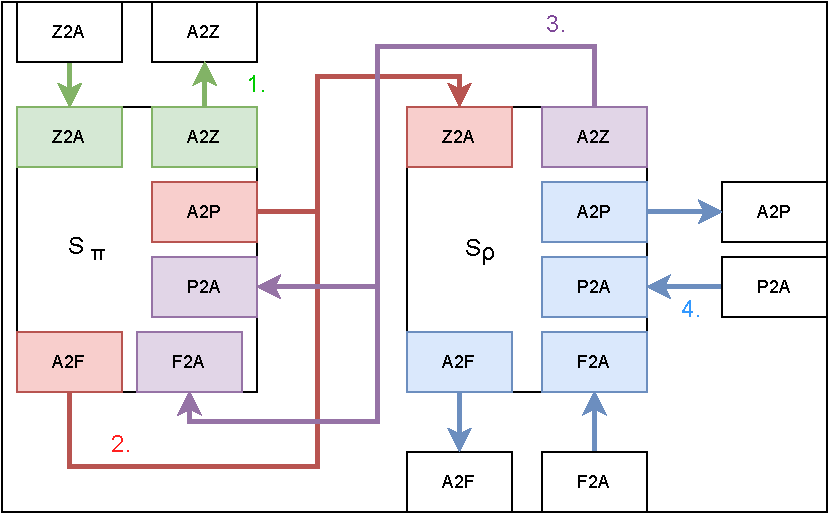
\includegraphics[scale=0.62]{figures/simcomp.pdf}
\caption{The composed simulators for $\F_1 \xrightarrow{\rho \circ \pi} \F_3$. The real world consists of $(\rho \circ \pi, \F_1)$. Inputs from \Z are for $\F_1$ and dummy parties interacting with $\F_1$, which \SIM{\pi} is equipped to handle. Outputs from \SIM{\pi} are for $\F_2$ and dummy parties of $\F_2$ which \SIM{\rho} is equipped to handle. FInally, outputs from \SIM{\rho} are for $\F_3$ and dummy parties of $\F_3$, which is just the ideal world in Theorem~\ref{thm:composition}.}
\label{fig:simcomp}
\end{figure}

%\begin{lstlisting}[basicstyle=\small\BeraMonottFamily, mathescape, frame=single]
%m = recv $\$$p2a ;
%case m (
%  P2A(pid, msg) =>
%   	case msg (
%      Committed =>
%        h = sample r k ;
%        send $\$$z2a P2A2Z(pid, (h)) ;
%      Open(b) =>
%	    x = sample r k ;
%        send $\$$z2a P2A2Z(pid, SMsg(b, x)) ;
%\end{lstlisting}

%When the committer is corrupt, the simulator has to do more work. 
%The key point that makes commitment in the RO model realizable is that \Z acquires commitment to give to the corrupt committer from \Fro through \A. 
%In th ideal world, the simulator recrods all the (key,value) pairs generated by its simulation of \Fro and therefore can always determine the bit \Z is committed to.
%When \Z queries \Sim with \inline{Z2A2F(SHash(b + x))} it stores the value and generates a hash value for it and returns it to \Z. 
%When instructed to give input to the corrupt party the simulator, \Sim gives input \inline{A2P(1, Commit(b))} where $b$ is the bit whos hash was requested.
%
%There is a unique edge case where \Z give some random bit sequence to \S as the commitment which wasn't generated by the random oracle. 
%In this case \S chooses a bit at random annd passes \inline{A2P(1, Commit(b))} to the protocol wrapper where $b$ is randomly selected.
%When prompted to open the commitment, \S does nothing as the real world receiver would fail to confirm whether the commitment corresponds to the bit $b$.




%\subsection{Ideal World}
%We described the functionality \Fcom in detail in Section~\ref{sec:execuc} as well as the functionality wrapper construction around it.
%We now describe how we implement ideal world (dummy) parties.

%We first describe at a high-level, the conversion happening within the functionality wrapper for \Fcom with the \inline{commit} message sent by the sender.
%When the wrapper receives the \inline{commit} message, the functionality wrapper executes the following:
%\begin{lstlisting}[basicstyle=\small\BeraMonottFamily, frame=single, mathescape]
%$\tg{(* l1 : list[pid \textasciicircum sender] *)}$
%case $\$$p2f (
%  yes => 
%    pid = recv $\$$p2f ; msg = recv $\$$p2f ;
%    case msg (
%      Commit(b) => 

%        $\$$ch_ = get_channel_by_pid pid $\$$l1 $\$$l2 ... ;
%        $\$$ch_.commit ;
%        send $\$$ch_ b ;
%        $\$$l2' <- append $\$$ch_ $\$$l2 ;
%\end{lstlisting}
%The wrapper also spawns a process to read from each of \Fcom's outgoing channels, case analyze on their value and send out the corresponding functional message to the protocol wrapper.

%The \msf{execUC} function in Figure~\ref{lst:execuc} accepts some number of type parameter which it spawns the main channels of the protocol with. 
%Most important out of these channels is the types governing communication between \Z and \A and between \Z and the protocol wrapper.
%If the types for these channel in both worlds aren't the same, even the import token expected, then it is trivial for an environment to distinguish the two worlds.
%It suffices to specify the import type parameters (\inline{p2f}, \inline{f2p}, \inline{z2p}, etc.) to \inline{execUC}.
%\paragraph{The Ideal World Execution}
%We summarize the message types in use by describing the type parameters to the ideal world execution.
%For the ideal, \inline{execUC} is invoked as follows (refer to the \inline{execUC} definition in Figure~\ref{lst:execuc} for what each of the parameters refers to):
%\begin{lstlisting}[basicstyle=\small\BeraMonottFamily, frame=single, mathescape]
%$\Type$ z2amsg[a][b] = Z2A2P of pid ^ a 
%                     | Z2A2F of b ;
%$\tg{(* ideal world *)}$
%execUC[K1,K2][comf2p][comp2f][comp2f][comf2p]
%  [comf2p][comp2f][comf2a][coma2f][rof2a][roa2f]
%  [rof2p][rop2f]
%\end{lstlisting}
%%$\tg{(* real world *)}$
%%execUC[K1,K2][comf2p][comp2f][rop2f][rof2p]
%%  [rof2p][rop2f][comf2a][coma2f][rof2a][roa2f]
%%  [rof2p][rop2f]
%Notice that the message types over \inline{p2z} and over \inline{p2f} are the same, because the ideal world parties are dummy parties which simply forward the messages to \Fcom.
%The type parameters for the adversary in the ideal world, though, still take the form of the types of \Fro.
%This is because the inputs \Z gives to both worlds (the dummy adversary in the real world) is intended for \Fro when communicating with the functionality through the adverasary or through corrupt parties 
%
%The party inputs from \inline{a2p} in the ideal world are intended for \Fcom, not \Fro, so they are of the same type \inline{comp2f}.
%Similarly, output from corrupt parties to the adversary in the ideal world is the same as output from \Fcom, and, therefore the message type is the same as \inline{comf2p}.
%The messages type parameters are wrapped in channel-specific types as well.
%For example, the channel \inline{z2a} is typed as follows:
%\begin{lstlisting}[basicstyle=\small\BeraMonottFamily, frame=single, mathescape]
%type z2amsg[a][b] = Z2A2P of pid ^ a
%                      | Z2A2F of b ;
%#z_to_a: comm[z2amsg[a2p][a2f]]
%$\tg{(* a2p=rop2f, a2f=roa2f in execUC above*)}$
%\end{lstlisting}
%
%\paragraph{Ideal Protocol}
%The ideal world protocl is a dummy party which forwards all messages to the functionality. 
%The message content from \inline{z2p} and \inline{p2f} is the same in the ideal world, but it is wrapped in different parameteric typed when it is sent from the \inline{z} or \inline{p}.
%As shown below the messages themselves are the same (\inline{comp2f} but typed differently (\inline{z2pmsg} vs \inline{p2fmsg}):
%\begin{lstlisting}[basicstyle=\small\BeraMonottFamily, frame=single, mathescape]
%$\Type$ z2pmsg[a] = Z2P of pid ^ a ;
%$\Type$ p2fmsg[a] = P2F of pid ^ a ;
%#z_to_p: comm[z2pmsg[comp2f]] ;
%#p_to_f: comm[p2fmsg[comp2f]] ;
%\end{lstlisting}
%The protocol wrapper only needs to forward the message unaltered but using a different type construtor. 

%The ideal functionality \Fcom is the same one introduced in Figure~\ref{fig:fcom} in Section~\ref{sec:nomosuc}. 
%In FIgure~\ref{lst:fcom} we present the Nomos definition of the same functionality and provide the channel types in FIgure~\ref{fig:fcomtypes}.
%We elide some of the clutter of acquiring and releasing shared channels in the form of: \texttt{\$p2f $\leftarrow$ acquire \#p\_to\_f} for clarity. 
%Wherever a linear channel like \texttt{\$p2f} is used it is in fact an acquired shared channel \texttt{\#p\_to\_f}.
%
%The key difference to note between \Fcom and its Nomos version is that the functionality is split up into two processes rather than compressed into one.
%This design decision is required because of how Nomos cycles between processes in a round-robin fashion and the communicator design.
%Therefore, processes must recurse when there is no message to be read and move to the next processes after the first expected message is received--in this case the \msf{P2FCommit(b)} message.
%
%
%\begin{figure}
%\centering
%\msf{type} \msf{Ip2f} = \msf{P2FCommit} of \msf{Bit} | \msf{P2FOpen}
%
%\msf{type} \msf{If2p} = \msf{F2PCommit} | \msf{F2POpen} of \msf{Bit}
%
%\msf{type} \msf{Ip2f} = \msf{SCommit} of Bit | \msf{SOpen}
%
%\msf{type} \msf{If2p} = \msf{RCommit} | \msf{ROpen} of Bit
%
%\msf{type} \msf{Rp2f} = \msf{SHash} of \msf{Int} | \msf{Send} of \msf{pid} \textasciicircum \msf{pid} \textasciicircum \msf{Int}
%
%\msf{type} \msf{Rf2p} = \msf{Pre} of \msf{Int} | \msf{RHash} of \msf{Int} | \msf{MSG} of \msf{pid} \textasciicircum \msf{pid} \textasciicircum \msf{Int}
%
%\caption{Types for the channels in the ideal world for \Fcom. Notice that Ip2f and If2p is the type of the channels \msf{z2p} and \msf{p2z} as they much match for both worlds and the ideal world parties simply forward messages to the functionality. The \msf{p2f} and \msf{f2p} channels are specific to the real and ideal world as the functionalities are not the same. Hence the real-world \msf{p2f} is typed with \msf{Rp2f} for the random oracle and the ideal world \msf{p2f} is typed with \msf{Ip2f} for \Fcom.}
%\label{fig:fcomtypes}
%\end{figure}
%
%\begin{figure*}
%\begin{lstlisting}[basicstyle=\small\BeraMonottFamily]
%proc F_code:
%  (s: sid), (k: Int), (rng: [Bit]), (clist: list[Int]),
%  (#p_to_f: comm[pid ^ Ip2f]{Ip2fn}), (#f_to_p: comm[pid ^ If2p]{If2pn}),
%  (#a_to_f: comm[Ia2f]{Ia2fn}), (#f_to_a: comm[If2a]{If2an})  |- ($ch: FtOE) =
%{
%  case $p2f (
%    yes =>	
%      pid, msg = recv $p2f ;
%      get $pwf {Ip2fn} ;
%      case msg (
%        P2FCommit(b) =>	
%          if pid == 1
%          then
%            send F2PCommit $f2p ;
%            pay {If2pn} $f2p ;
%            $ch <- F_com_open s k rng clist #p_to_f #f_to_p b ;
%          end
%      )
%   | no =>  
%       $ch <- F_code s k rng clist #p_to_f #f_to_p ;
%  )
%}
%
%proc F_code_open:
%{
%  case $p2f (
%    yes =>	
%      pid, msg = recv $p2f ;
%      get $p2f {0} ;
%      case msg (
%        P2FOpen =>	
%          if pid == 1
%          then
%            send F2POpen(b) $f2p ;
%            pay {0} $f2p ;
%            $ch <- 1 ;
%          end
%      )
%   | no =>
%       $ch <- F_code_open s k rng clist #p_to_f #f_to_p b ;
%  )
%}
%\end{lstlisting}
%\end{figure*}
%
%The real world protocol for commitment follows a simple communication patter:
%\begin{enumerate}
%\item On input bit $(\msf{P2FCommit}\ b)$ from the environment, the committer queries the random oracle with the message $(\msf{SHash}\ b | r)$ where $r \xleftarrow{\$} \{0,1\}^k$.
%The returned ``hash value'' is sent to the receiver as the commitment.
%\item On input \msf{P2FOpen} from \Z, the committer sends $(\msf{Send}\ p_L\ b\ r)$ to the receiver.
%\item The receiver checks that the commitment is correct be querying \Fro in the same way and asserting that the has returned $(\msf{RHash}\ h)$ is the same as the one sent by $p_C$.
%\item \todo{the type of Rf2p is kind of wrong so need to correct it}
%\end{enumerate}
%
%We provide only a simulator for the dummy adversary as that guarantees a simulator for all adversaries required our emulation definition.
%The simulator for commitment is relatively simple so we only provide a high-level description here and leave the full simulator code to the appendix.
%The simulator internally simulats the random oracle by maintaining a table of key-value pairs that it can control entirely.
%If the committer is corrupt:
%\begin{enumerate}
%\item The simulator can not determine the bit \Z wants to commit to so selects a random bit when activatd by the environment and gives it as input to the corrupted committer.
%\item When it's asked to open the commitment it simply forwards the request to the corrupt committer and stops.
%\end{enumerate}
%If the receiver is corrupt:
%\begin{enumerate}
%\item When activated by the receiver with (\msf{F2PCommit}), the simulator generates some random string $h$ to represent the commitment, stores it, and sends ($\msf{P2A}\ \msf{MSG}(p_C, p_R, h)$) to \Z.
%\item When it receives ($\msf{F2POpen}\ b$) from the receiver, it returns $(\msf{P2A}\ \msf{MSG}(p_C, p_R, b, r)$ to \Z where $r$ is a randomly generated sequence keeping the pair $(b | r, h)$ as the corresponding entry in the table.
%\item When activated by \Z to check the commitment, \Sim simply returns the commitment hash or creates a new one.
%\end{enumerate}
%
%\paragraph{Simulator Well-Matched}
%It is immediately obvious that the constructed simulator is well-typed if the dummy adversary is well-typed with the given type parameters.
%The simulator receives 1 import token per activation from \Z which suffices to simulated \Fro internally. 
%Subsequently, \Sim keeps all of the import it receives, and, therefore when one of the partiesis corrupt a simple bounding polynomial can be given as:
%\[
%	T_{\Dummysim}(n) = T_{\Fro}(n) + O(1)
%\]
%where $T_{\Fro}$ is a satisfying polynomial for \Fro. The additional constant factor simply accounts for sending messages to the corrupt parties.
%Therefore,
%\begin{gather}
%	\forall \Z, \langle \Z \leftrightarrow \DA \rangle \Rightarrow \langle \Z \leftrightarrow \Dummysim \rangle
%\end{gather}
%
%
%\begin{figure*}
%\begin{lstlisting}[basicstyle=\BeraMonottFamily]
%(* Z2P interface *)
%type Ip2f = P2FCommit of Bit | P2FOpen ;
%type If2p = F2PCommit | F2POpen of Bit ;
%
%(* Ideal World *)
%type Ip2f = SCommit of Bit | SOpen ;
%type If2p = RCommit | ROpen of Bit ;
%
%type Ia2f = 0 ;
%type If2a = 0 ;
%
%type Ia2p = Ip2f ;	(* crupt input is same as z2p *)
%type Ip2a = If2p ;
%
%(* Real World *)
%type Rp2f = SHash of Int | Send of pid ^ pid ^ Int ;
%type Rf2p = Pre of Int | RHash of Int | MSG of pid ^ pid ^ Int ;
%
%type Ra2f = A2Hash of Int ;
%type Rf2a = Hash2A of Int ;
%
%type Ra2p = Rp2f ;
%type Rp2a = Rf2p ;
%
%(* the import here is given as those for the dummy adversary in the real world *)
%p2zn <- 0 ; z2pn <- 1 ;
%a2zn <- 0 ; z2an <- 1 ; 
%
%Rf2pn <- 0 ; Rp2fn <- 1 ;
%Rp2an <- 0 ; Ra2pn <- 1 ;
%Rf2an <- 0 ; Ra2fn <- 1 ;
%
%If2pn <- 0 ; Ip2fn <- 0 ;
%Ip2an <- 0 ; Ia2pn <- 0 ;
%I
%
%(* channels *)
%#z_to_p <- comm[pid ^ Ip2f]
%#p_to_z <- comm[pid ^ If2p]
%#z_to_a <- comm[ z2d[Ra2p][Ra2f] ] ;
%#z_to_z <- comm[ d2z[Rp2a][Rf2a] ] ;
%
%
%(* Real World exec PI *)
%execUC[Ip2f][If2p][Rp2f][Rf2p][Rp2a][Ra2p][Rf2a][Ra2f][a2z][z2a]
%	  {p2zn}{z2pn}{f2pn}{p2fn}{p2an}{a2pn}{f2an}{a2fn}{a2zn}{z2an}
%
%(* Ideal world exec PHI *)
%execUC[If2p][Ip2f][Ip2f][If2p][Ip2a][Ia2p][If2a][Ia2f][a2z][z2a]
%	  {p2zn}{z2pn}
%
%
%
%
%
%
%\end{lstlisting}
%\end{figure*}


The type system in NomosUC helps to identify when the amount of potential that a functionality requires isn't satisfied by the bounding polynomia given.
We illustrate this point using the $\F_{\msf{map}}$. 
The functionality maintains a list that parties can append to the end of or read from.


%\caption{The $\mathcal{F}_{\msf{comm}}$ commitment ideal functionality in Nomos. The types for the sender and receiver channel define what inputs they can give to the functionality and what messsages are sent from the functionality back to the receiver.}
%\label{fig:nomos:commitment}
%\end{figure*}

\subsection{Formal Description of the NomosUC Language}

The core calculus of the NomosUC language is based on
\emph{session types}: a type discipline for communication-centric programming
based on message passing via channels. Session-typed channels describe and
enforce the protocol of communication among processes. The base system of
session types is derived from a Curry-Howard interpretation~\cite{caires2010session}
of intuitionistic linear logic~\cite{girard1987linear}.
As a result, purely linear
propositions can be viewed as resources that must be used \emph{exactly
once} in a proof yielding the sequent $A_1, \ldots, A_n \vdash C$
where $A_1, \ldots, A_n$ are linear antecedents, while $C$ is the linear
succedent. Under this correspondence, a process term $P$ is assigned to
the above judgment and each hypothesis as well as the conclusion is
labeled with a \emph{channel}:
\[
x_1 : A_1, \ldots, x_n : A_n \vdash P :: (z : C)
\]
The resulting judgment states that process $P$ \emph{provides} a service
of session type $A$ along channel $z$, \emph{using} the services of session
types $A_1, \ldots, A_n$ provided along channels $x_1, \ldots, x_n$
respectively. We mandate all channel names to be distinct for the judgment
to be \emph{well-formed}. The antecedents are often abbreviated to $\D$.

The operational semantics for session-typed programs are formalized as a
system of \emph{multiset rewriting rules}~\cite{cervesato2009relating}.
We introduce semantic objects $\proc{c}{P}$ and $\msg{c}{M}$ describing
process $P$ (or message $M$) providing service along channel $c$.
Remarkably, in this formulation, a message is just a particular form of process,
thereby not requiring any special rules for typing; it can be typed just as processes.

Formally, the typing judgment for processes in NomosUC is written as
$k \semi \Tokens \semi \Psi \semi \D \entailpot{q}{q'} P :: (x : A)$.
Here, $\Psi$ denotes the functional data structures and $\D$ collects the
session-typed channels along with an optional write token $\wt$
(to resolve non-determinism in the semantics).
The process is denoted by $P$ that offers channel $x$ of type $A$.
Finally, token context $\Tokens$ contains the total and current ($=$ received - sent)
tokens of each type contained by the process and $k$ is the globally known \emph{security parameter}.
Similar to import tokens, the natural number annotations $q$ and $q'$ on the turnstile
denote the total and current potential stored in the process.
We also extend the semantic objects to $\proc{c}{w, P}$ and $\msg{c}{w, P}$
where work counter $w$ stores the work performed by process $P$ (resp.
message $M$).
We will gradually explain each component of the language, initiating
with the basic system of session types.
For simplicity of exposition, we will display the yet unexplained
parts of the system in blue.

The Curry-Howard correspondence gives each linear logic connective an
interpretation as a session type.
In this article, we restrict to a subset of these connectives that
are sufficient for our language and purposes.
We follow a detailed description of each of these session type constructors.

An example process is given below, implementing \Fcom according to the \m{sender} and
\m{receiver} types.
\Fcom 
As an illustration, consider the $\Fcom$ process that is connected
to both $S$ and $R$ in Figure~\ref{fig:profcom}.
\begin{figure}
\centering
\begin{lstlisting}[basicstyle=\footnotesize\BeraMonottFamily, frame=single, mathescape]
$\nproc$ $\tm{Fcom}$: 
  (k: $\tgr{int}$), (rng: [Bit]), (sid: SID), ($\$$S: sender), ($\$$R: receiver)  |- ($\$$fc: 1) =
{
  $\ncase$ $\$$S (
    commit => b = $\nrecv$ $\$$S ; $\$$R.commit ;
              case $\$$S (
                open => $\$$R.open ; $\nsend$ $\$$R b ;
}
\end{lstlisting}
\caption{The process code for \Fcom.}
\label{fig:procfcom}
\vspace{-4mm}
\end{figure}

Here, $\Fcom$ is the name of the process, and $S$ and $R$ are the names
of channels \emph{used} by $\Fcom$, while \inline{fc} is the channel \emph{provided}
by $\Fcom$.
The used channels with their types are written to the left of the turnstile
($\vdash$) while the offered channel and type are written on the right.
This is analogous to function definitions where used channels correspond to
arguments, while offered channel corresponds to the result.
In the case of $\Fcom$ the offered channel \inline{fc} is not used. This is
a result of how we design functionalities in NomosUC, which we explain later.

The process first case analyzes on channel $S$ branching on the
message received.
Since there is only one choice $\mb{commit}$, we only have one
branch in the definition.
$\Fcom$ then receives the bit $b$ (line 3) on $S$, followed by sending the
commit message on channel $R$ (line 4).
Once $\Fcom$ receives the $\mb{open}$ message on $S$, it sends the
$\mb{open}$ message on $R$ (line 6), followed by the bit $b$ (line 7).

\paragraph*{\textbf{Internal Choice}}
The internal choice $\ichoice{\ell : A_\ell}_{\ell \in L}$ constructor
is an $n$-ary labeled generalization of the additive disjunction $A \oplus B$.
A process that provides $x : \ichoice{\ell : A_\ell}_{\ell \in L}$ can send
any label $k \in L$ along $x$ and then continue by providing $x : A_k$. The
corresponding process is written as $(\esendl{x}{k} \semi P)$, where
$P$ is the continuation that provides $A_k$. This typing is formalized
by the \emph{right rule} $\oplus R$ in linear sequent calculus. The
corresponding client branches on the label received along $x$ as specified
by the \emph{left rule} $\oplus L$.
\begin{mathpar}
  \footnotesize
  \infer[{\oplus}R]
  {\B{k \semi \Tokens \semi \Psi} \semi \wt, \D \entailpot{\B{q}}{\B{q'}} (\esendl{x}{k} \semi P) ::
    (x : \ichoice{\ell : A_\ell}_{\ell \in L})}
  {(k \in L) \qquad \B{k \semi \Tokens \semi \Psi} \semi \D \entailpot{\B{q}}{\B{q'}} P :: (x : A_k)}
\end{mathpar}
\begin{mathpar}
  \footnotesize
  \infer[{\oplus}L]
  {\B{k \semi \Tokens \semi \Psi} \semi \D, (x : \ichoice{\ell : A_\ell}_{\ell \in L})
    \entailpot{\B{q}}{\B{q'}} \ecase{x}{\ell}{Q_\ell}_{\ell \in L} :: (z : C)}
  {(\forall \ell \in L) \qquad \B{k \semi \Tokens \semi \Psi} \semi \wt, \D, (x : A_\ell)
    \entailpot{\B{q}}{\B{q'}} Q_\ell :: (z : C)}
\end{mathpar}
Additionally, the provider should possess the write token to be able to send the
label $k$. Dually, the client receives the write token with the label to continue
execution.

Operationally, since communication is asynchronous, the process
$(\esendl{c}{k} \semi P)$ sends a message $k$
along $c$ and continues as $P$ without waiting for it to be received.
As a technical device to ensure that consecutive messages on a
channel arrive in order, the sender also creates a fresh continuation
channel $c'$ so that the message $k$ is actually represented as
$(\esendl{c}{k} \semi \fwd{c}{c'})$ (read: send $k$ along $c$ and
continue as $c'$). The provider substitutes $c'$ for $c$ enforcing
that the next message is sent on $c'$.
The work counter of the process remains unaltered, and the new message
is created with work $0$.
\begin{tabbing}
$(\oplus S) : \proc{c}{w, \esendl{c}{k} \semi P} \step$ \= $\proc{c'}{w, [c'/c]P},$\\
\> $\msg{c}{0, \esendl{c}{k} \semi \fwd{c}{c'}}$
\end{tabbing}
When the message $k$ is received along $c$, the client selects branch
$k$ and also substitutes the continuation channel $c'$ for $c$, thereby
ensuring that it receives the next message on $c'$. This implicit
substitution of the continuation channel ensures the ordering of the
messages.
The client process also collects the work performed by the message.
\begin{tabbing}
$(\oplus C) :$ \= $\msg{c}{w, \esendl{c}{k} \semi \fwd{c}{c'}},
\proc{d}{w', \ecase{c}{\ell}{Q_\ell}}$\\
\> $\qquad \step \proc{d}{w+w',[c'/c]Q_k}$
\end{tabbing}

\paragraph*{\textbf{External Choice}}
The dual of internal choice is \emph{external choice} $\echoice{\ell :
A_\ell}_{\ell \in L}$, the $n$-ary labeled generalization of the
additive conjunction $A \with B$. This dual operator simply reverses
the role of the provider and client. The provider process of
$x : \echoice{\ell : A_\ell}_{\ell \in L}$ branches on receiving a label
$k \in L$ (described in $\with R$), while the client sends this label
(described in $\with L$).
\begin{mathpar}
  \footnotesize
  \infer[\with R]
  {\B{k \semi \Tokens \semi \Psi} \semi \D \entailpot{\B{q}}{\B{q'}} \ecase{x}{\ell}{P_\ell}_{\ell \in L} ::
    (x : \echoice{\ell : A_\ell}_{\ell \in L})}
  {(\forall \ell \in L) \qquad \B{k \semi \Tokens \semi \Psi} \semi \wt, \D
    \entailpot{\B{q}}{\B{q'}} P_\ell :: (x : A_\ell)}
\end{mathpar}
\begin{mathpar}
  \footnotesize
  \infer[\with L]
  {\B{k \semi \Tokens \semi \Psi} \semi \wt, \D, (x : \echoice{\ell : A_\ell}_{\ell \in L})
    \entailpot{\B{q}}{\B{q'}} \esendl{x}{k} \semi Q :: (z : C)}
  {\B{k \semi \Tokens \semi \Psi} \semi \D, (x : A_k) \entailpot{\B{q}}{\B{q'}} Q :: (z : C)}
\end{mathpar}
Dual to internal choice, the client contains the write token which is
sent to the provider along with the label.
The operational semantics rules are just the inverse of internal choice,
and therefore skipped for brevity.

\paragraph*{\textbf{Termination}}
The type $\one$, the multiplicative unit of linear logic, represents
termination of a process, which (due to linearity) is not allowed to use
any channels. A terminating process offering on $x : \one$ simply
closes channel $x$ while the client waits for this close message to arrive.
\begin{mathpar}
  \footnotesize
  \infer[{\one}R]
  {\B{k \semi \Tokens \semi \Psi} \semi \wt \entailpot{\B{q}}{\B{q'}} \eclose{x} :: (x : \one)}
  {\B{q = 0}}
  \and
  \infer[{\one}L]
  {\B{k \semi \Tokens \semi \Psi} \semi \D, (x : \one) \entailpot{\B{q}}{\B{q'}} (\ewait{x} \semi Q) :: (z : C)}
  {\B{k \semi \Tokens \semi \Psi} \semi \wt, \D \entailpot{\B{q}}{\B{q'}} Q :: (z : C)}
\end{mathpar}
Similar to internal choice, the closing process transfers the write
token to its waiting client along with the close message.
Additionally, the terminating process does not store
any potential since it cannot take any further execution steps.
% Operationally, the provider converts into a closing message
% with no continuation since the offered channel terminates.
% \begin{tabbing}
% $(\one S) : \proc{c}{\eclose{c}} \step \msg{c}{\eclose{c}}$ \\
% $(\one C) : \msg{c}{\eclose{c}}, \proc{d}{\ewait{c} \semi Q} \step
% \proc{d}{Q}$
% \end{tabbing}

% The provider receives the branching label $k$ sent by the provider. Both
% processes perform appropriate substitutions to ensure the order of messages
% sent and received is preserved.
% \[
% \begin{array}{lll}
% (\with S) & \proc{d}{\esendl{c}{k} \semi Q} \step \msg{c'}{\esendl{c}{k}
% \semi \fwd{c'}{c}}, \proc{d}{[c'/c]Q} & \fresh{c'} \\
% (\with C) & \proc{c}{\ecase{c}{\ell}{Q_\ell}_{\ell \in L}},
% \msg{c'}{\esendl{c}{k} \semi \fwd{c'}{c}} \step \proc{c'}{[c'/c]Q_k}
% \end{array}
% \]

\paragraph*{\textbf{Exchanging Functional Data}}
Communicating a \emph{value} of the functional fragment along a channel
is expressed at the type level by adding the following two session types.
\begin{center}
\begin{minipage}{0cm}
\begin{tabbing}
$A ::= \ldots \mid \tau \arrow A \mid \tau \product A$
\end{tabbing}
\end{minipage}
\end{center}
Here, $\tau$ describes a functional type, e.g. $\m{int}, \m{bool}, \tau \; \m{list}$, etc
(we assume the language contains standard functional types).
The type $\tau \arrow A$ prescribes receiving a value of type $\tau$
with continuation type $A$, while its dual $\tau \product A$ prescribes
sending a value of type $\tau$ with continuation $A$. The corresponding
typing rules for arrow ($\arrow R, \arrow L$) are given
below (rules for $\product$ are inverse).
\begin{mathpar}
  \footnotesize
  \infer[\arrow R]
  {\B{k \semi \Tokens} \semi \Psi \semi \D \entailpot{\B{q}}{\B{q'}}
  \erecvch{x}{v} \semi P :: (x : \tau \arrow A)}
  {\B{k \semi \Tokens} \semi \Psi, (v : \tau) \semi \wt, \D \entailpot{\B{q}}{\B{q'}}
  P :: (x : A)}
  %
  \and
  %
  \inferrule*[right = $\arrow L$]
  {\B{r' = p+q'} \qquad
  \B{\Psi \share (\Psi_1, \Psi_2)} \qquad
  \Psi_1 \exppot{\B{p}} M : \tau \\
  \B{k \semi \Tokens} \semi \Psi_2 \semi \D, (x : A) \entailpot{\B{q}}{\B{q'}}
  Q :: (z_k : C)}
  {\B{k \semi \Tokens} \semi \Psi \semi \wt, \D, (x : \tau \arrow A)
  \entailpot{\B{q}}{\B{r'}} \esendch{x}{M} \semi Q :: (z : C)}
\end{mathpar}
As indicated in the $\arrow R$ rule, receiving a value $y : \tau$ on a channel
$x : \tau \arrow A$ adds it to the functional context $\Psi$. On the
other hand, sending (value of) expression $M$ on channel $x : \tau \arrow A$
requires that $M$ has type $\tau$ (third premise).
The premises indicated in blue describe how potential is divided across
the functional and session-typed layers and will be described next.
Intuitively, the potential in functional context $\Psi$ is \emph{shared}
between $\Psi_1$ and $\Psi_2$ (second premise); $\Psi_1$ is used to type
$M$ while $\Psi_2$ is passed on to the continuation $Q$.

\subsection{Expressing ITMs With Session Types}
Despite the seemingly stuctured nature of execution in UC, the framework is meant to capture arbitrary connections, communication patterns, or configurations of ITMs. 
In this section we highlight a common pattern in UC that requires additional machinery to be express with session types.

The pattern emerges from the following code: a machine $P$ either writes to another machine $Q$ or is written to by $Q$. 
At first glance, it is a trivial scenario, but we encounter a problem trying to encode this with a single session type.
A example are machines $P$ and $Q$ which execute as follows:
\begin{itemize}
	\item An external machines flips a bit and activates either $P$ or $Q$.
	\item If $P$ is activated it writes to $Q$ and the execution terminates. 
	\item Otherwise, if $Q$ is activated, it writes a message to $P$, $P$ writes something back, and the execution terminates.
\end{itemize}
A single type between $P$ and $Q$ would have to allow either of the two parties to write on the channel, but session types require it to be statically known.

If we try to separate communication between $P$ and $Q$ into two uni-directional channels, we end up with Figure~\ref{fig:pandq}, and can express the session type for each of the channels:
\begin{center}
\parbox{0cm}{
\begin{tabbing}
$\m{PtoQ} = \ichoice{\mb{``one''}: int \tensor 1}$ \\
$\m{QtoP} = \echoice{\mb{``one''}: int \tensor \ichoice{\mb{``end''}: int \tensor 1}}$
\end{tabbing}}
\end{center}

This approach, however, poses another problem. 
Channels are only created by a process offering them, and a process can only offer a single channel.
Without adding any additional processes, $P$ must offer a channel to $Q$ and $Q$ offer one to $P$. 
Each of them becomes both a provider and a client to the other, and provider/client ambiguity is not allowed in Nomos. 
Logically, one process must have spawned the other, and such a cycle would be impossible to realize.

In order to capture this communication, and, in general, to break all possible cycles while still making meaningful use of session types, we propose a construction like Figure~\ref{fig:newpandq}.
We wrap each of $P$ and $Q$ in shell code, call them $S_P$ and $S_Q$, which spawn two dummy proceses to offer each of the channels of type \m{PtoQ} and \m{QtoP} to $P$ and $Q$.
The arrows within each shell represent the direction of communication rather than a provider-client relationship. 
In reality, any of the process can offer any of the channels as long as it doesn't result in a cycle.
\begin{figure}
	\begin{subfigure}{0.3\textwidth}
	\centering
	
\includegraphics[scale=0.4]{figures/p_and_q.png}
	\caption{Two channels can define capture communication, but provider-client cycles are not allowed in NomosUC.}
	\label{fig:pandq}
	\end{subfigure}
	~ \ \ \ \ 
	\begin{subfigure}{0.6\textwidth}
	\centering
	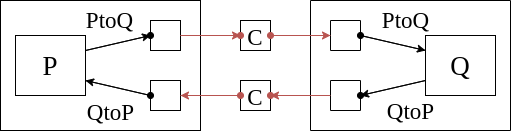
\includegraphics[scale=0.4]{figures/new_p_and_q.png}
	\caption{We can realize the left be intermediating communication with communicators. The direction of messages from $P$ to $Q$ still suggest a cycle but the communicator is provider (dot) to \emph{both} shell codes.}
	\label{fig:newpandq}
	\end{subfigure}
	\caption{Two ITM configurations. One possible with ITMs (left) and one realized in NomosUC (right). Arrows indicate direction of messages and the dot indicates the provider of the channel.}
\end{figure}
Communication between $S_1$ and $S_2$ along channels they each offer results in another cycle. 
Therefore, we break the cycle by intermediating their communication through a \emph{communicator}.
The communicator avoids cycles by offered a \emph{shared channel} rather than the typical linear channel.

\paragraph*{\textbf{Shared Channels}}
\todo{Here I'm not too sure on whether this is enoug information or if it's correct.}
Linear channels are exclusive to the parent and child that are at their endpoints.
Balzer et al.~\cite{balzer2017manifest} proposed a \emph{shared} extension of session types which allows them to capture more natural programming scenarios where cyles naturally occurrs (ring network, dining philosophers, etc.).
Shared channels are still restricted to one provider but can be used by multiple clients to communicate with the provider. 
They introduce non-determinism that isn't present in UC where many clients can be attempting to communciate with the same provider, however, NomosUC borrows the write token from ILC to ensure activation and control are always with only on process at a time.

\paragraph*{\textbf{Communicators}}
Communicators act as channel buffers that two parties can use to communicate to each other.
The shared type of the communicators is given by 
\begin{center}
\parbox{0cm}{
\begin{tabbing}
$\m{comm[a]} = \up \echoice{$\=$\mb{SEND}: \m{a} \product \m \down \m{comm[a]},$\\
\>$\mb{RECV}: \ichoice{$\=$\mb{yes}: \m{a} \product \down \m{comm[a]},$\\
\>\>$\mb{no}: \down \m{comm[a]}}}$
\end{tabbing}}
\end{center}
The $\up$ and $\down$ operations around the session type indicate that it is \emph{shared}, and they denote a \emph{critical section} analogous to traditional concurrency controls like the mutex.
The type suggests that one party can send a message to the communicator, the communicator, buffers the message, and responds with it when asked to \m{RECV} is from a another process.

Returning to the initial example of $P$ and $Q$, although the contruction appears excessive, it is generic and can intermediate communication between any pair of processes in NomosUC. 
It allows us to continue to meaningfully use session types and avoid worrying about cyclical provider/client relationships for the remainder of this paper.
As we show in Section~\ref{sec:execuc}, communicators also help intermediat eocmmunication between each of the main processes of the execution.

\section{The rest of nomos? don't know how to break up this section to include the above.}
\paragraph*{\textbf{Import Tokens}}
A defining aspect of NomosUC is the representation of import tokens in the type system.
This enables a static reasoning of the import mechanism in NomosUC.
To this end, we introduce a novel token context $\Tokens$
in the process typing judgment to denote the real and virtual tokens.
This context contains the information on the total and current tokens
of each type and the \emph{security parameter}.
Before we explain the token context we first motivate the need for virtual tokens
It is a common technique in UC, especially in simulators, to internally run, or simulate, 
the code of other ITIs. In NomosUC, we wish to enable the same sandbox running of processes,
but its channels may have import requirements. It doesn't make sense to
send real import to such a process, because, intuitively the internal process should use the
import and, therefore, potential available to the ``host'' process~\footnote{As far as resource-contraints go, simulating a process should be no different from natively executing its code.}. Therefore, in 
order to satisfy the types of internally simulated processes we introduce a virtual 
tokens construction. 
By default, every process contains a unique real token type $K_0$
and corresponding number of total and current tokens $n$ and $n'$ resp.\
denoted by $K_0 \hookrightarrow (n, n')$.
There is no mechanism to create a real token; they can only be passed on to
a process during its creation, or be exchanged between processes during communication.
Virtual tokens, on the other hand, can be created (under certain conditions,
see below) by a process.
However, all tokens follow a \emph{token hierarchy}: $K_0 \to K_1 \to K_2 \to \ldots K_m$
such that we can only use tokens of type $K_i$ to withdraw tokens of type
$K_{i+1}$~\footnote{ITIs in UC can have arbitrary simulation depth, i.e. a process simulates another process which simulates another process. Despite this, we can statically define the token heirarchy because it is statically known the maximum simulation depth of any process in the UC execution.}.
In addition, we use a global function $\GlobalF$ as the connection
rate between two successive token types.

To maintain well-typedness of a process, an implicit side condition is
that the token context must always be \emph{valid}.
This involves ensuring that if the context contains $m'$ current tokens of type
$K_i$, it can only contain at most $\GlobalF(m,k)$ total tokens of type
$K_{i+1}$. The inductive rules for validity of a token context are below.
\begin{mathpar}
  \infer
  {K_0 \hookrightarrow (t_0, t_0') \;\; \m{valid}}
  {}
  \and
  \infer
  {k \and \Tokens, K_{i+1} \hookrightarrow (t_{i+1}, t_{i+1}')\;\; \m{valid}}
  {\Tokens\;\; \m{valid} \and
  K_{i} \hookrightarrow (t_i, t_i') \in \Tokens \and
  t_{i+1} \leq \GlobalF(t_i',k)}
\end{mathpar}
Since validity of a token context is a side condition, we mandate
that it is implicitly satisfied by all the process typing rules
presented in our paper.
From an implementation point-of-view, this validity check only
needs to be performed when the token context changes (in the
rules that follow).

As a first step in introducing program notation for import tokens, we need 
syntax for creating new tokens of a given token type.
We call this construct $\m{withdrawToken} \; K_i \; n \; K_{i+1}$.
\begin{mathpar}
  \inferrule*[right=$\m{tok}$]
  {k \semi \Tokens, K_{i+1} \hookrightarrow (t_{i+1} + n, t_{i+1}' + n) \semi
  \Psi \semi\wt, \D \entailpot{\B{q}}{\B{q'}} P :: (x : A)}
  {k \semi \Tokens, K_{i+1} \hookrightarrow (t_{i+1}, t_{i+1}') \semi \Psi \semi \wt, \D \entailpot{\B{q}}{\B{q'}} \hspace{4em} \\
    \hspace{5em}\m{withdrawToken} \; K_i \; n\; K_{i+1}  \semi P :: (x : A)}
\end{mathpar}
The above construct generates $n$ new tokens of type $K_{i+1}$ and adds
them to both the total and current count for $K_{i+1}$ in the token
context $\Tokens$.
The implicit side condition of the validity of the token context ensures
that $t_{i+1} + n \leq \GlobalF(t_i',k)$ where $K_i \hookrightarrow (t_i, t_i') \in \Tokens$.
If this side condition fails, the above construct would fail to typecheck.

In addition, we also introduce two dual constructs for exchanging tokens
between processes.
To this end, we first introduce two new type constructors.
\begin{center}
\begin{minipage}{0cm}
\begin{tabbing}
$A ::= \ldots \mid \tpaypot{A}{r : K} \mid \tgetpot{A}{r : K}$
\end{tabbing}
\end{minipage}
\end{center}
The provider of $x : \tgetpot{A}{r : K}$ is required to receive
$r$ import tokens of type $K$ from the client using the construct
$\eget{x}{r : K}$. Dually, the client needs to pay this import
using the construct $\epay{x}{r : K}$.
The corresponding typing rules are
\begin{mathpar}
  \footnotesize
  \infer[\getpot R]
  {k \semi \Tokens, K_i \hookrightarrow (t_i, t_i') \semi \Psi \semi \D \entailpot{\B{q}}{\B{q'}} \eget{x}{r : K_i} \semi P ::
  (x : \tgetpot{A}{r : K_i})}
  {k \semi \Tokens, K_i \hookrightarrow (t_i, t_i'+r) \semi \Psi \semi \wt, \D \entailpot{\B{q}}{\B{q'}} P :: (x : A)}
  %
  \and
  %
  \infer[\getpot L]
  {k \semi \Tokens, K_i \hookrightarrow (t_i, t_i'+r) \semi \Psi \semi \wt, \D, (x : \tgetpot{A}{r : K_i}) \entailpot{\B{q}}{\B{q'}}
  \epay{x}{r : K_i} \semi P :: (z : C)}
  {k \semi \Tokens, K_i \hookrightarrow (t_i, t_i') \semi \Psi \semi \D, (x : A) \entailpot{\B{q}}{\B{q'}} P :: (z : C)}
\end{mathpar}
In the rule $\getpot R$, process $P$ storing $(t_i, t_i')$ import tokens of type $K_i$
receives $r$ additional $K_i$ tokens adding it to the current token counter, thus
the continuation executes with $(t_i, t_i'+r)$ tokens of type $K_i$.
Note that validity of token context is trivially satisfied in this case since the
process is gaining import tokens.
%
In the dual rule $\getpot L$, a process containing $(t_i, t_i'+r)$ tokens of type $K_i$
pays $r$ units along channel $x$ leaving $(t_i, t_i')$ import tokens of type $K_i$ with
the continuation.
In this case, the validity of the token context establishes that $t_{i+1} \leq \GlobalF(t_i',k)$,
a condition that is necessary for successful typechecking.
The typing rules for the dual constructor $\tpaypot{A}{r : K}$
are the exact inverse.
Similar to prior rules, the sender transfers the write token $\wt$
along with the potential to the receiver.

The need for virtual tokens in UC arises because machines often simulate
other machines as part of their construction. The program notation for \msf{withdrawToken}
does not require an inverse to exchange tokens \textit{back} from type $K'$ to $K$.
The reason is that virtual tokens only exist to allow re-use of existing processes 
and satisfy their types. Type $K$ tokens are not deducted when new ones of type $K'$ 
are created is because, in reality, siulating a process by calling it or simply running
its code natively should be equivalent in cost. Therefore, there is also no need to 
include an inverse of \msf{withdrawToken} which exchanges from $K'$ to $K$.

\paragraph*{\textbf{Potential}}
The main purpose of import tokens is to bound the number of execution steps of ITMs.
We achieve that purpose in NomosUC by introducing the notion of \emph{potential}.
Potential is an abstract quantity represented by a natural number stored
within each process.
To take an execution step, a process consumes \emph{one} unit of potential.
Therefore, the total potential stored in a process upper bounds the total
number of execution steps that will ever be taken by the process.
Furthermore, potential is represented syntactically, thus providing a
static upper bound on the execution cost.
Since execution cost needs to eventually connect to the import tokens, all
we need is a mechanism to generate potential using import tokens.
To this end, we introduce a novel construct $\m{genPot} \; r$.
\begin{mathpar}
  \inferrule*[right=$\m{pot}$]
  {q+r \leq \GlobalF(t_{\depth}',k) \and K_{\depth} \hookrightarrow (t_{\depth}, t_{\depth}') \in \Tokens \\\\
  k \semi \Tokens \semi \Psi \semi \wt, \D \entailpot{q+r}{q'+r} P :: (x : A)}
  {k \semi \Tokens \semi \Psi \semi \wt, \D \entailpot{q}{q'} \m{genPot} \; r \semi P :: (x : A)}
\end{mathpar}
A process initially storing $(q, q')$ potential units generates $r$ potential so that
the continuation contains $(q+r, q'+r)$ potential units.
Note, however, that the maximum potential allowed is bounded by the number of import tokens
a process contains.
To this end, we introduce a \emph{token depth}: $\depth$ that signifies the number of token
types that exist in the token hierarchy.
Thus, when generating potential, the typechecker verifies that the total new potential (i.e., $q+r$)
is bounded by $\GlobalF(t_{\depth}',k)$ where $(t_{\depth}, t_{\depth}')$ is the number of tokens
of type $K_{\depth}$, the highest token in the hierarchy.

The purpose of introducing potential into NomosUC is to bound the
number of execution steps.
Therefore, we introduce the $\etick{r}$ construct that consumes $r$
potential from the stored process potential $q$, and the continuation remains with
$p = q-r$ units, as described in the rule below.
\begin{mathpar}
  \footnotesize
  \infer[\m{tick}]
  {k \semi \Tokens \semi \Psi \semi \wt, \D \entailpot{q}{q'+r} \etick{r} \semi P :: (x : A)}
  {k \semi \Tokens \semi \Psi \semi \wt, \D \entailpot{q}{q'} P :: (x : A)}
\end{mathpar}
NomosUC is equipped with a cost instrumentation engine that automatically
inserts a $\etick{1}$ construct before each primitive operation.
This enables us to simulate the cost model that counts the total number of
execution steps.
However, since ticks are not tied directly to the type system, the programmer
can modify the cost model to only count the resource they are interested in
(e.g., message exchange, process spawns, etc.).

% \begin{mathpar}
%   \D_1 \equiv_Z \D_2 \\
%   \D \overset{(import, potential, cost)}{\vDash} P :: \D' \\
%   A \equiv B \\
%   \infer[]
%   {\vars \vdash \D_1, (x : A) \equiv \D_2, (x : B)}
%   {\vars \vdash \D_1 \equiv \D_2 \and \vars \vdash A \equiv B}
% \end{mathpar}

\paragraph*{\textbf{Shared Channels}}
Until now, we have only described the linear fragment of session types
in Nomos.
Unfortunately, this fragment imposes a strong restriction on programs.
The only provision to spawn new processes is when a parent process creates a new
child process, and uses an exclusive linear channel to communicate with the child.
Thus, any two processes connected by a channel inherently maintain this parent-child
relationship.
Intuitively, this leads to a linear tree-like hierarchy among the processes,
thus preventing a cycle in the process graph.

Unfortunately, this restriction precludes practical programming scenarios
where process topologies indeed have a cyclic dependency (e.g. ring networks,
dining philosophers, etc.).
Recognizing this limitation, Balzer et al.~\cite{balzer2017manifest} proposed
a \emph{shared} extension of session types that allows arbitrary process topologies.
The types are extended as follows:
\begin{center}
\begin{minipage}{0cm}
\begin{tabbing}
$A_L ::= \down A_S \mid \ldots \text{(all linear types $A$ so far)}\ldots$\\
$A_S ::= \up A_L$
\end{tabbing}
\end{minipage}
\end{center}
We have found this extension exceedingly helpful in the design and implementation
of cryptographic protocols.

Shared session types impose an \emph{acquire-release} discipline on processes; 
a client must acquire the channel offered by a shared process to interact with it
and must release this channel after the interaction.
The corresponding typing rules are
\begin{mathpar}
  \footnotesize
  \infer[\up L]
  {k \semi \Tokens \semi \Psi \semi \wt, \D, (x : \up A_L)
  \entailpot{q}{q'} \eacquire{y}{x} \semi Q :: (z : C)}
  {k \semi \Tokens \semi \Psi \semi \D, (y : A_L)
  \entailpot{q}{q'} Q :: (z : C)}
  %
  \and
  %
  \infer[\up R]
  {k \semi \Tokens \semi \Psi \semi \D \entailpot{q}{q'}
  \eaccept{y}{x} \semi P :: (x : \up A_L)}
  {k \semi \Tokens \semi \Psi \semi \wt, \D \entailpot{q}{q'} P :: (y : A_L)}
\end{mathpar}
The $\up L$ rule describes a client acquiring a shared channel $x$
and obtaining a private linear channel $y$ along which it can communicate
with the corresponding acquired process.
Correspondingly, the $\up R$ rule describes the shared process
accepting the acquire request and creating the fresh linear channel $y$.
The release-detach rules corresponding to the $\down$ type constructor
are exact dual of acquire-accept.

An important caveat here is that shared channels can introduce non-determinism
in the semantics.
The only source of non-determinism is that a shared process can latch on to
any of the acquiring clients.
To address this problem, we require that the acquiring client \emph{possess
the write token}.
Since write tokens are treated as a linear quantity, only one of the client can
possess it enabling only that process to acquire the shared channel.
Remarkably, this write token can resolve both read and write non-determinism
due to linearity of the channels.


\paragraph*{\textbf{Process Definitions and Sandboxing}}
Process definitions have the form
$\Psi \semi \D \entailpot{q}{q'} f\{\Tokens\} :: (x : A) = P$ where $f$
is the name of the process and $P$ its definition.
We parameterize the process $f$ with the number and type of
real tokens it would need.
All definitions are collected in a fixed global process signature $\Sg$.
Also, since process definitions are mutually recursive, it is required that
for every process in the signature is well-typed w.r.t. $\Sg$.
A new instance of a defined process $f$ can be spawned with
the expression $\procdef{f\{\Tokens\}}{\overline{y}}{x} \semi Q$
where $\overline{y}$ is a sequence of variables matching the
antecedents $\Psi$ and $\D$.
Sometimes a process invocation is a \emph{tail call}, written without
a continuation as $\procdef{f\{\Tokens\}}{\overline{y}}{x}$.
This is a short-hand for
$\procdef{f\{\Tokens\}}{\overline{y}}{x'} \semi \fwd{x}{x'}$ for a
fresh variable $x'$, that is, a fresh channel is created and
immediately identified with $x$.

An important note here is that NomosUC allows executing processes in
a \emph{sandbox}.
Therefore, a process invocation can either be \emph{regular} or in a
\emph{sandbox}.
Syntactically, we use the same term for both but the two invocations
are distinguished via the token type passed into the call.
For a regular call, the parent process passes in a real token type,
while for a sandboxed call, a virtual token type is passed in.
We have a similar distinction for $\m{pay}$ and $\m{get}$ expressions:
if a real token is passed into these terms, it's a regular token
exchange; if a virtual token is passed in, it's a sandboxed $\m{pay}$
and $\m{get}$.

\subsection{Preservation and Progress}
The main type safety theorems that exhibit the deep connection between our type
system and the operational semantics are the usual \emph{type
preservation} and \emph{progress}, sometimes called \emph{session
fidelity} and \emph{deadlock freedom}, respectively.

To exhibit these theorems, we first need to introduce semantic objects
$\proc{c}{w, P}$ and $\msg{c}{w, M}$.
The former (resp. latter) denotes a process (resp. message) executing
expression $P$ (resp. $M$) offering channel $c$ and having performed
work $w$ so far.
The work counter keeps track of execution steps taken by a process,
giving rise to the following semantics rule:
\begin{tabbing}
  $(\m{tick}) : \proc{c}{w, \etick{r} \semi P} \step \proc{c}{w+r, P}$
\end{tabbing}
A multiset of such semantic objects communicating with each other
is known as a \emph{configuration}.
A configuration is typed w.r.t. a signature providing the type declaration
of each process.
A signature $\Sg$ is \emph{well formed} if
(a) every type definition $V = A_V$ is \emph{contractive},
and (b) every process definition
$\Psi \semi \D \vdash f \{\Tokens\} = P :: (x : A)$ in $\Sg$
is well typed according to the process typing judgment, i.e.
$\Tokens \semi \Psi \semi \D \vdash P :: (x : A)$.
 
A key question then is how to type these configurations.
Since they consist of both processes and messages, they
both \emph{use} and \emph{provide} a collection of channels.
Another goal with the type safety theorems is to establish a connection
between the statically determined import tokens of a process,
its total potential, and the dynamically evolving work counters
that account for the total number of execution steps.
We use the following judgment to type a configuration.
\[
\D_1 \overset{(T, Q)}{\underset{W}{\vDash}} \config :: \D_2
\]
It states that the configuration $\config$
uses the channels in the context $\D_1$ and provides the channels in
the context $\D_2$.
In addition, $T$ and $Q$denote the total number of real tokens
potential contained in a configuration.
Similarly, $W$ denotes the total work performed by a configuration.
All these quantities are computed by adding the individual tokens,
potential, and work of each semantic object.
\begin{figure}[t]
\begin{mathpar}
\infer[\m{empty}]
{\D \overset{(0, 0)}{\underset{0}{\vDash}} (\cdot) :: \D}
{}
\and
\infer[\m{compose}]
{\D_0 \overset{(T_1+T_2, Q_1+Q_2)}{\underset{W_1+W_2}{\vDash}} (\config_1 \; \config_2) :: \D_2}
{\D_0 \overset{(T_1, Q_1)}{\underset{W_1}{\vDash}} \config_1 :: \D_1 \qquad
\D_1 \overset{(T_2, Q_2)}{\underset{W_2}{\vDash}} \config_2 :: \D_2}
\and
\infer[\m{proc}]
{\D, \D_1 \overset{(t, q)}{\underset{w}{\vDash}} \proc{c}{w, P} :: (\D, (c : A) )}
{\Tokens, K_0 \hookrightarrow t \semi \cdot \semi \D_1 \entailpot{q} P :: (c : A)}
\and
\infer[\m{msg}]
{\D, \D_1 \overset{(t, q)}{\underset{w}{\vDash}} \msg{c}{w, M} :: (\D, (c : A) )}
{\Tokens, K_0 \hookrightarrow t \semi \cdot \semi \D_1 \entailpot{q} M :: (c : A)}
\end{mathpar}
\caption{Typing rules for a configuration}
\label{fig:config_typing}
\end{figure}

The configuration typing judgment is defined using
the rules presented in Figure~\ref{fig:config_typing}.
%
The rule $\m{empty}$ defines that an empty configuration
is well-typed with $(T, Q, W) = (0, 0, 0)$ and uses and
provides the same set of channels.
The $\m{compose}$ rule combines two configurations by canceling out
the common channels and adding the individual tokens, potential, and work.
The $\m{proc}$ rule creates a configuration out of a single process
and uses its tokens, potential, and work as the annotations for the
configuration.
Similarly, the $\m{msg}$ rule creates a configuration out of a single message.

\begin{theorem}[Type Preservation]
\label{thm:preservation}
Suppose we have a well-typed configuration
$\D \overset{(T_1, Q_1)}{\underset{W_1}{\vDash}} \config_1 :: \D'$ such
that there exists a polynomial $\mathfrak{p}$ such that $\mathfrak{p}(T_1) \geq Q_1+W_1$.
If $\config_1 \step \config_2$, then there exist $T_2$, $Q_2$, and $W_2$ such
that $\D \overset{(T_2, Q_2)}{\underset{W_2}{\vDash}} \config_2 :: \D'$,
and $\mathfrak{p}(T_2) \geq Q_2+W_2$.
\end{theorem}
\begin{proof}
  By case analysis on the transition rule, applying inversion to the
  given typing derivation, and then assembling a new derivation of
  $\dc$.
\end{proof}

A process or message is said to be \emph{poised} if it is trying to
communicate along the channel that it provides.  A poised process is
comparable to a value in a sequential language. A configuration is
poised if every process or message in the configuration is poised.
Conceptually, this implies that the configuration is trying to communicate
externally, i.e. along one of the channel it provides.
The progress theorem then shows that either a configuration can take a
step or it is poised.  To prove this I show first that the typing
derivation can be rearranged to go strictly from right to left and
then proceed by induction over this particular derivation.

\begin{theorem}[Global Progress]
\label{thm:progress}
\mbox{}
If $\cdot \overset{(T, Q)}{\underset{W}{\vDash}} \config :: \D$ then either
\begin{enumerate}
\item[(i)] $\config \mapsto \config'$ for some $\config'$, or
\item[(ii)] $\config$ is poised.
\end{enumerate}
\end{theorem}
\begin{proof}
By induction on the right-to-left typing of $\config$ so that either
$\config$ is empty (and therefore poised) or
$\config = (\dc\; \proc{c}{w, P})$ or
$\config = (\dc\; \msg{c}{w, M})$. By induction hypothesis, $\dc$ can
either take a step (and then so can $\config$), or $\dc$ is poised.  In
the latter case, I
analyze the cases for $P$ and $M$, applying multiple steps of
inversion to show that in each
case either $\config$ can take a step or is poised.
\end{proof}


%\subsection{UC Communicators} \label{sec:communicators}
%% all the processes conncted together leads to a cycle of linear channels ==> Z <--> P so here we use a communicator 
%The UC execution connects the protocol to the environment in both directions of communication.
%This poses a technical challenge where, if linear channels are used, the resulting topology contains a cycle of linear channels: the environmtne offers a channel to the wrapper and the wrapper to the environment.
%Such cycles violate type preservation because a client is acquiring its client~\ref{dasnomos}.
%Therefore, we use a message buffers called communicators which offered shared channels that both ends of the communication can use.
%Communicators are used in the main UC execution in Section~\ref{sec:execuc} to connect the main processes together, as well as within the \partywrapper. 
%
%A communicator has a \emph{sender} and a \emph{receiver}. 
%The shared channel offered by the communicator has the following polymorphic session type:
%\begin{tabbing}
%  $\mi{stype} \; \m{comm[K][msg]\{n\}} =$\\
%  \quad $\up \tgetpot{}{n+1: K} \echoice{$\=$\mb{push} : \m{msg} \arrow
%  \down \m{comm[msg]},$\\
%  \>$\mb{pop} : \ichoice{$\=$\mb{yesmsg} : \m{msg} \product \down \tpaypot{}{n: K} \m{comm[msg]},$\\
%  \>\>$\mb{nomsg} : \down \m{comm[msg]} }}$
%\end{tabbing}
%
%One illustration of the use of shared session types is a \emph{communicator}.
%We use communicators as message buffers between two arbitrary processes: a
%\emph{sender} and a \emph{receiver}.
%The communicator is connected to both the sender and the receiver using a shared
%channel.
%
%Intuitively, the communicator receives \emph{push} requests from the sender followed
%by receiving a message and stores them internally.
%Analogously, the communicator receives \emph{pop} requests from the receiver,
%and responds appropriately with the message if one is stored inside the communicator.
%Formally, a communicator has the following polymorphic session type
%\begin{tabbing}
%  $\mi{stype} \; \m{comm[K][msg]\{n\}} =$\\
%  \quad $\up \tgetpot{}{n+1: K} \echoice{$\=$\mb{SEND} : \m{msg} \arrow
%  \down \m{comm[msg]},$\\
%  \>$\mb{RECV} : \ichoice{$\=$\mb{yes} : \m{msg} \product \down \tpaypot{}{n: K} \m{comm[msg]},$\\
%  \>\>$\mb{no} : \down \m{comm[msg]} }}$
%\end{tabbing}
%The $\up$ indicates that it is a shared channel that must be \emph{acquired} by a process in order to send something over it.
%
%The sender can $\mb{SEND}$ a message into the communicator, and the receiver can periodically try to $\mb{RECV}$ a message from it.
%If there is a message, it responds with $\mb{yes}$, the message of the parameterized type $\m{msg}$, and the import sent with it.
%Note that the communicator retains one unit of import from every message. 
%It needs at least one because it may be activated a polynomial number of times, and, therefore a constant amount of potential is insufficient. 
%At the end of activation, the channel is released with $\down$, and another process can acquire it.

\subsection{Discussion on Realizing Import}
Our adaptation of the import mechanism to resource-aware session types concretizes some parts of the import mechanism like the run-time budget and adds new mechanisms
to facilitate common UC design pattersn such as simulation and virtualization of machines. 
It's important to validate our realization of the import mechanism by ensuring that it faithfully provides the same guarantees.
Furthermore, in this section we discuss existing pitfalls and drawbacks of prior mechanisms that import was created to over come, and assert that our implementation steers clear of them as well.

An important part of our discussion must focus around our sandboxing technique and ensuring that it does not provide a pathway for a process to run infinitely.
The infinite runs problems is a persistent issue in existing length-of-input based approaches to polynoimal time.
It naturally appears in our sandboxing mechanism by the continual creation of new virtual token types. Following from the intent of sandboxing, the NomosUC rule for a valid token context ensures that all virtual token types  \todo{ finish this by deciding which rule to update: \inline{genPot} or \inline{withdrawTokens}}

%\begin{itemize}
%\item Identify design decisions like concretizing potential, sandboxing and virtualizing with withdrawTokens, the valid token context rule, the type system in general
%\item Identify polytime concerns that need to be discussed in the context of our polytime design
%	\begin{itemize}
%	\item is PPT efficiently recognizable?
%	\item address the infinite runs problem and make sure it isn't allowed here with particular attention paid to withdrawTokens and infinite virtualizations
%	\item the type system guarantees we don't have a case where, given some polynomial, a machine just halts mid execution so we avoid any additional information that an environment can use to distinguish based on execution timing in both word
%	\end{itemize}
%\item end with the virtualization point and tie that into proposition 7 and the universal turing machine that can simulate the UC execution. This goes a long way in assuring PPT notion in NomosUC, even thought we aren't dealing exactly with ITMs here.
%\end{itemize}

%The type $\m{comm}$ is parameterized by the type $\m{msg}$, i.e., the type of
%messages in the buffer, and import type parameter, i.e. the amount of import tokens sent with
%the message. 
%The type initiates with an $\up$ denoting that $\m{comm}$ is a shared session type.
%The type prescribes that the communicator needs to be acquired by the sender (or receiver)
%for further interaction.
%Such an acquire-release discipline is automatically enforced by the shared session type.
%Once acquired, the communicator can either receive $\mb{push}$ (from sender) or
%$\mb{pop}$ requests (from receiver).
%In the former case, the communicator receives a message of type $\m{msg}$ and $n+1:K$ import tokens, and
%then detaches from the client using the dual $\down$ operator.
%In the latter case, the communicator checks if it internally contains a message
%for the receiver.
%If yes, the communicator replies with the $\mb{yesmsg}$ label followed by sending
%the message (the $\product$ constructor) and $n:K$ import tokens.
%Otherwise, the communicator replies with the $\mb{nomsg}$ label.
%In either case, the communicator then detaches from the client matching the $\down$
%operator.
%Internally, the communicator stores these messages in a first-in-first-out order.

%It is important to note that our communicators need at least 1 token of import 
%to use themselves to handle a potentially polynomial number of activations. 
%Therefore, it requires $n+1$ units of import from the sender and sends the intended
%$n$ tokens to the receiver when requested.

%The communicator is also the perfect opportunity to implement an unreliable
%message buffer that can drop or reorder messages.
%All we would need to do is change the internal implementation of the communicator
%\emph{without} changing the offered session type.
